%! TEX root = 'main.tex'

\section{\name Design}
\label{sec:ktoctou-design}

This section presents the design of \name.  The core of \name includes two key components, the system module and the hypervisor. The system module intercepts the system's page fault handler to process SMAP and relevant exceptions, which is the protection's main logic.  The lightweight hypervisor puts the system into the virtual machine when loaded. Its primary use is to confine the system-wide feature SMAP into specific processes.

\subsection{System Module}

The system module's core functions include enabling SMAP, recovering from SMAP exceptions, protecting pages, and solving read/writes conflicts. We describe each technique as follows.

\textbf{\textit{Monitoring Kernel to Userspace Access. }} The biggest challenge we confront is how to monitor the kernel-to-userspace behavior efficiently. Accessing memory is such an ordinary operation so that no purposeful hardware feature is available for monitoring that.  We notice a rarely memtioned hardware feature SMAP. Its initial design prevents the attacker from tricking the kernel into getting shellcode or malicious data from userspace. When the kernel accesses a user address, the processor raises a page fault exception. This part accurately serves our purpose, so we want to leverage it in a novel way. 

However, not every aspect of this feature perfectly fits our exceptions. If in an ideal situation, the hardware should report on each kernel-to-userspace access and freeze the user memory at machine word granularity. In reality, SMAP only works on the page level, and the exception that it raised is fatal to the system, meaning the operating system should crash when it receives such exceptions.  We eventually find a way to recover it. We intercept the system's page fault handler to handle such exceptions, namely, vector 14 in the IDT. Since Windows does not support SMAP, we do not pass those exceptions to the kernel. Considering the violation of raising a SMAP exception is that the kernel accesses userspace, so puts the corresponding page into kernel space solves the exception. Otherwise, it is then too late to disable SMAP through CR4 or set EFLAGS.AC flag.


Putting a page into the kernel not only solves the exception but also protects the page. The user threads no longer can access it, which prevents the race condition between the kernel and user threads. However, it is overkill to protect the entire page and block benign reads and writes on the rest of the data. We discuss the read/writes conflicts in the following section.



\textbf{\textit{Solving Read Conflicts}}. For practical purposes, solving
read conflicts is essential. It is common to have multiple global
variables or multiple heap buffers share the same page. Therefore, when we protect an entire page, we block benign access to the rest of the data. It is especially unnecessary because reads do not harm security.

We solve the read conflicts by setting the protected page
back to userspace, allowing user threads to read. When user threads read a kernel-mode protected page, the processor raises an exception due to the privilege violation. Therefore our page fault handler gets the notification and sets the page back to userspace. Additionally, the page is also set with a read-only permit to ensure no write. ~\autoref{fig:pagestate} shows the transitions between kernel-mode and user-mode.  We record the original page information to handle various situations and correctly restore it at the end of the system call.


\begin{figure}[th]
  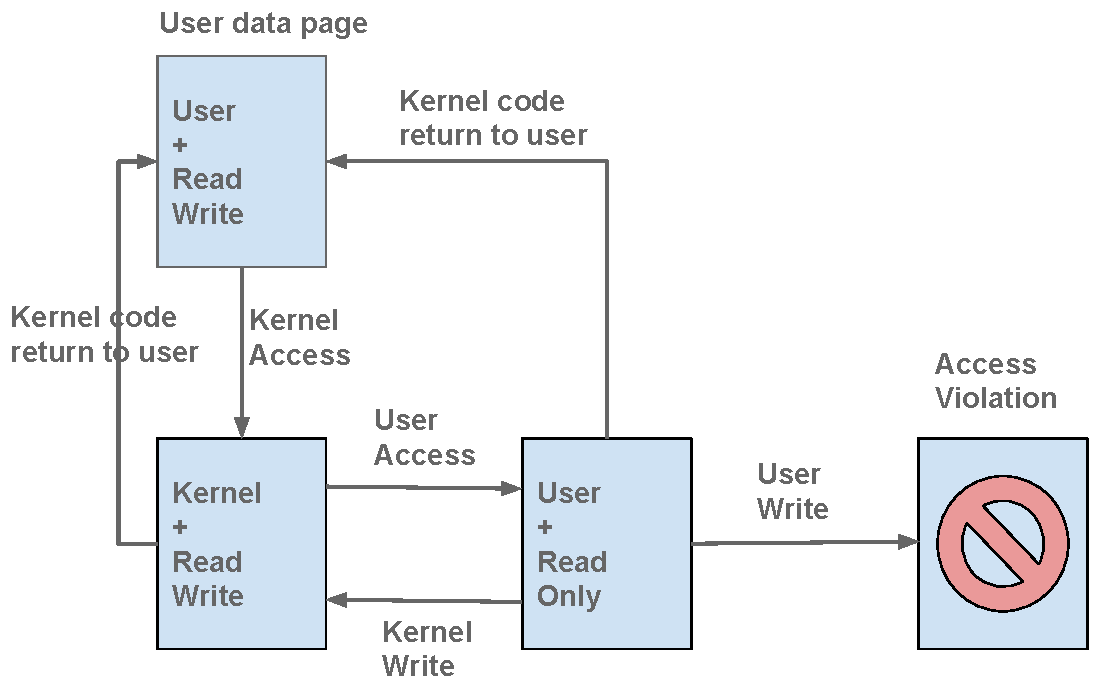
\includegraphics[width=0.30\textwidth]{figures/pagestate}
  \centering
  \caption{Page transits between kernel-mode and user-mode. A user page becomes a kernel page after the kernel access it. If user threads read this page, we change it back to user-mode with a read-only permit. Then this page is also then capable of triggering another SMAP exception if the kernel reaccesses it. Our page handler will suspend any thread that tries to write this page and keep checking the page's status to re-execute until the current system call ends or reaches a time limit. When the current system call ends, this page will be set back to user-mode with its original permits. Thus, the write thread is also released. }
  \label{fig:pagestate}
\end{figure}



\textbf{\textit{Page Attribute Transition.}}  The modifications on the page attributes are essential to this mitigation. Because changing a user page to kernel-mode is the primary method of protection.  Moreover, to solve reads conflicts, we need to change the page back and forth between kernel-mode and user-mode. 

First, we need to locate the page's Page Table Entry (PTE). As mentioned in~\autoref{sec:ktoctou-background}, with paging, every page in the virtual memory has an entry in the page table.  As shown in~autoref{fig:pte}, the User/Supervisor decides whether this is a kernel page or a user page. Set if it is a user page, otherwise a kernel page.


\begin{figure}[th]
  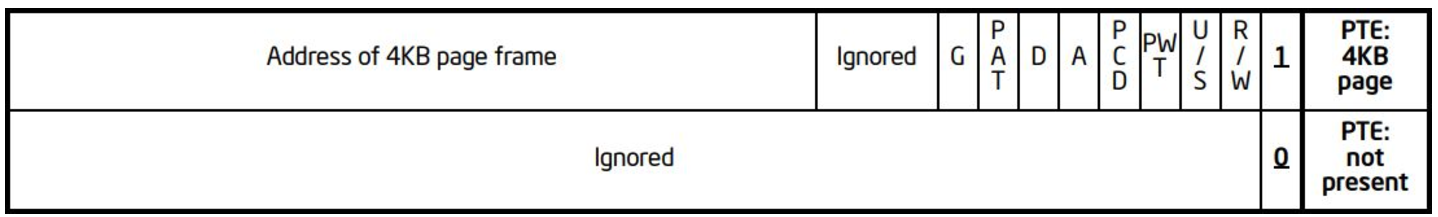
\includegraphics[width=0.47\textwidth]{figures/pte2}
  \centering
  \caption{\textbf{Bit 0} (Present): \textbf{0} indicates an invalid page. \textbf{U/S} (User/Supervisor): \textbf{0} user-mode accesses are not allowed to the page referenced by this entry. \textbf{R/W}: \textbf{0} writes are not allowed to the page.}
  \label{fig:pte}
\end{figure}



We obtain various information in the context of the page fault
handler to find the corresponding PTE. The CR2 register stores the faulting virtual address. Regarding SMAP, it is the user address that the kernel accessed. The CR3 register stores the physical address
of the current page table base. The trap frame in the kernel stack contains the error code, CS: EIP, SS: ESP, and EFLAGS, which describes the processor context when the exception happens.

Changing the U/S bit in the PTE makes the user page becomes a kernel page. It is counterintuitive because we usually have the impression that the virtual address between 0x80000000 to 0xFFFFFFFF is the kernel space on Windows 32-bit system. However, there is the Current Privilege Level (CPL) field in the CS segment. The processor maintains this 2-bit field to equal the processor's current privilege level. Meantime, the U/S bit in the PTE decides whether the unprivileged code can access it. Traditionally, we consider the memory space that only the most privileged code (CPL:00) can run as the kernel space. Indeed, it is a considerably complicated mechanism involving more data structure in the processor's microarchitecture, out of this paper's scope. In essence, the U/S bit decides whether the page is a kernel page or a user page, even the virtual address is below 0x80000000.



\begin{figure}[th]
  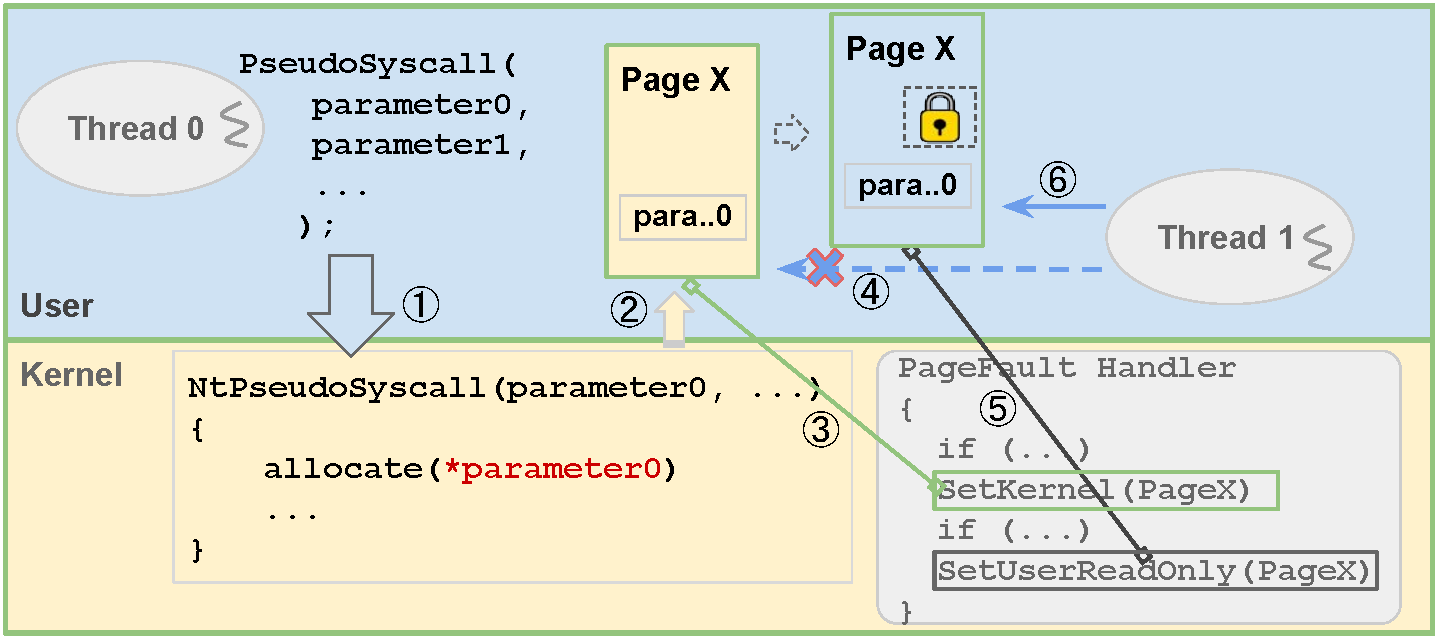
\includegraphics[width=0.47\textwidth]{figures/denyuserwrite3}
  \centering
  \caption{\texttt{\textcircled{1}} User thread 0 invokes a system call with parameters. \texttt{\textcircled{2}} The kernel fetches one of the parameters from userspace hence triggers a SMAP exception. \texttt{\textcircled{3}} Our page fault handler converts the page into kernel-mode to protect it. \texttt{\textcircled{4}} Another user thread 1 tries to read the protected page and triggers an exception due to privilege violation.  \texttt{\textcircled{5}} Again, our page fault handler processes the exception and converts the protected page back to user-mode with a read-only permit. \texttt{\textcircled{6}} The faulting instruction re-execute, and the user thread successfully read the data without knowing the previous exception.}
  \label{fig:denyuserwrite}
\end{figure}



~\autoref{fig:denyuserwrite} shows the mitigation convert a low address user page into a kernel page. It is a common situation where user programs invoke a system call and provide parameters. After that, if a user thread accesses a protected page, the processor raises an exception due to the privilege violation. The page fault handler converts this page to user-mode and read-only.


\textbf{\textit{Solving Write Conflicts.}} Unlike the read conflicts, we can not make the page writable at any time. Even the write on the rest of the data is benign. Subject to the x86 architecture, the protection has to base on page granularity. We have to make sure that no user-mode threads write the entire page during the system call. However, we can make them wait then write it after the system call. More specifically, once the write raises an exception, we suspend the thread until the current system call ends. We will discuss why it is possible to suspend a thread inside the page fault handler shortly after.


\begin{figure}[th]
  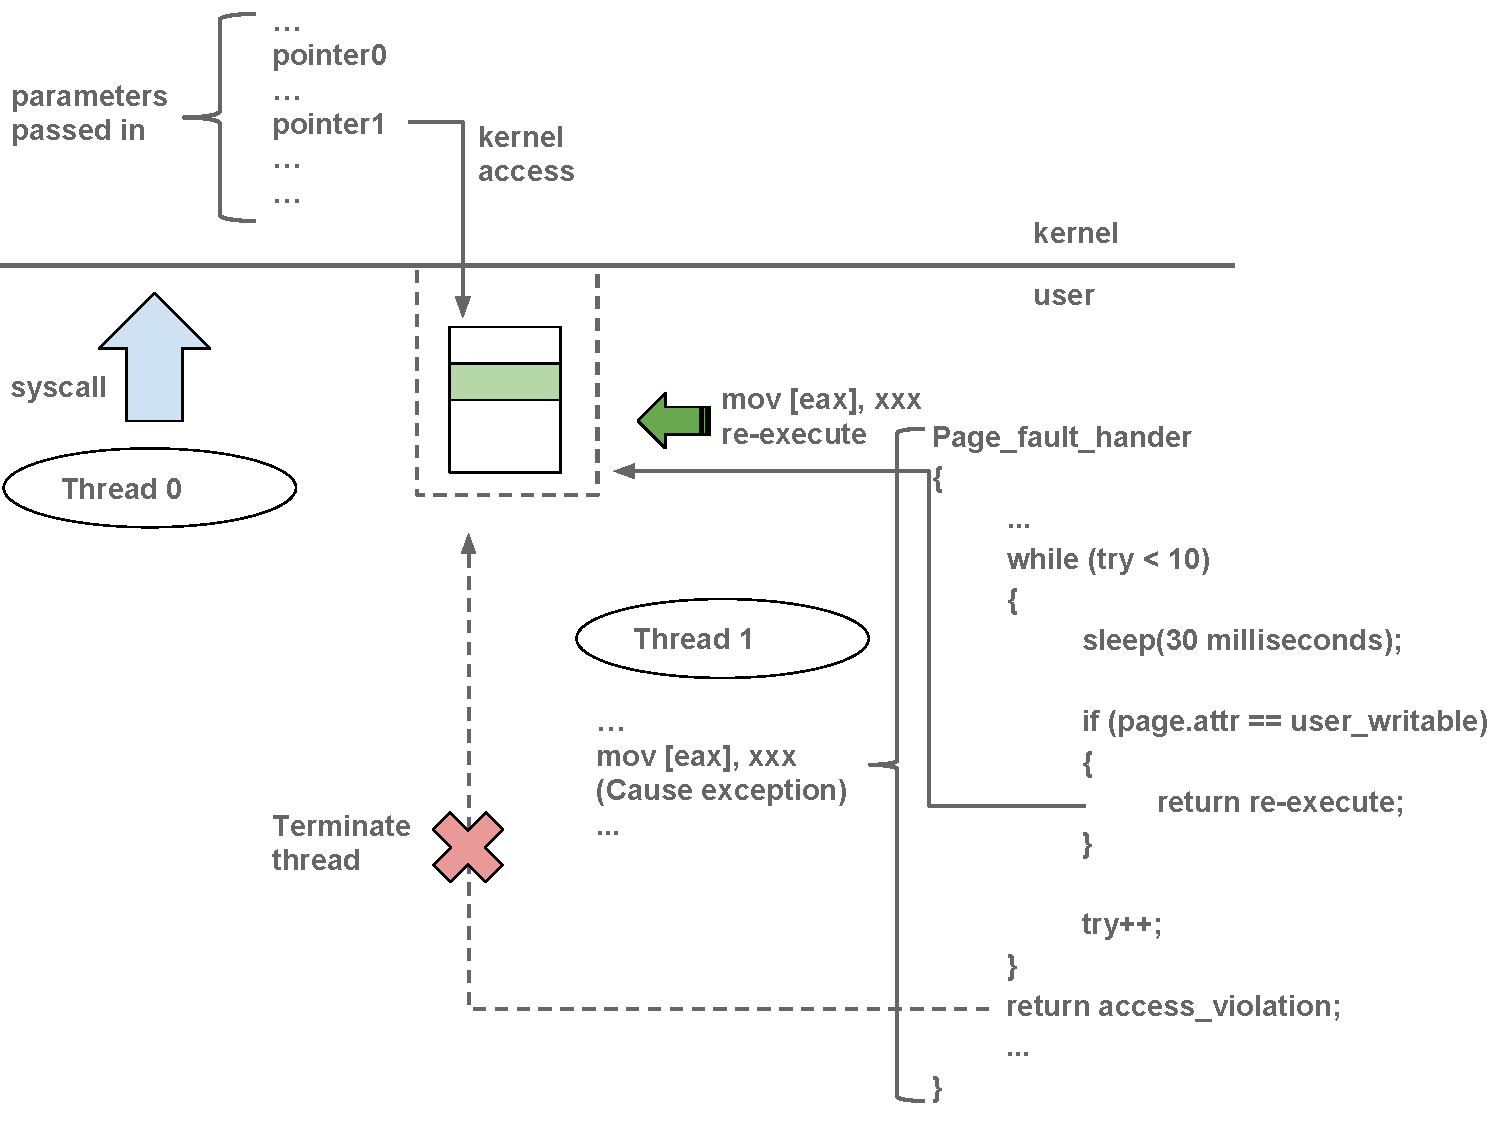
\includegraphics[width=0.47\textwidth]{figures/reexecute}
  \centering
  \caption{We take the delayed access solution when handling a write conflict. Thread one sleeps for a short time in the exception handler, letting the operating system schedule. Recheck the current status when it wakes up. Reexecute the faulting instruction if the protected page is released. Otherwise, wait for the next turn. Moreover, to avoid endless waiting, which may cause a deadlock, the thread will be terminated if it reaches the time threshold.}
  \label{fig:reexecute}
\end{figure}


As shown in ~\autoref{fig:reexecute}, thread 0 invokes a system call with parameters.  \name protects the corresponded page into kernel space once the kernel fetches those parameters. Afterward, thread 1 writes the page, which raises another page fault exception. Inside the handler, \name calls a kernel function, \texttt{KeDelayExecutionTread()}, that suspend the current thread. The thread wakes up periodically to check the page's status. If the page is released, it finishes the exception, re-executes the faulting instruction. Otherwise, \name terminates the thread to prevent any deadlock.

%\subsection{The Differences Between Interrupt and Exception}



\textbf{\textit{Interrupt and Exception.}} Thread suspending inside the page fault handler seems unusual because both interrupts and exceptions have their handler entries in the Interrupt Descriptor Table (IDT). However, the difference between them is essential.  An interrupt is an asynchronous event that is typically triggered by an I/O device. An exception is a synchronous event generated when the processor detects one or more predefined conditions while executing an instruction. Interrupts have a higher priority than the operating system's scheduler and most of the kernel components. Any job should not take too long inside the interrupt handler~\cite{msdnwatchdog}.  On the contrary, exceptions have the lowest priority in the kernel. In Windows' term, the Interrupt Request Level (IRQL) that the exception handler executes at is \texttt{PASSIVE\_LEVEL}. It means to call for thread scheduling is plausible.


%\subsection{Releasing Protected Pages}

%Whenever a syscall ends, all the protected page that related to it should be released. Their original attributes will be restored. The Thread Environment Block(TEB) is used to identify each thread within the current process. Each thread has its own TEB data and it's address is easy to locate by segment register FS. 

%We hook a Windows internal function in order to know when it's the end of the syscall. 

%\begin{comment}
%\begin{figure}[th]
%  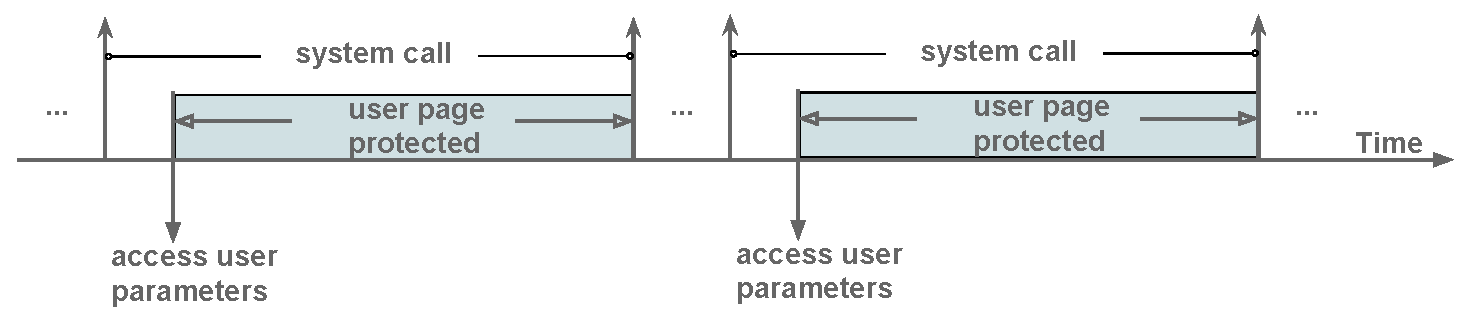
\includegraphics[width=0.40\textwidth]{figures/timeline}
%  \centering
%  \caption{The page protection period is within one system call cycle, this is based on the fact that kernel TOCTOU vulnerability does not happen across system calls.}
%  \label{fig:timeline}
%\end{figure}
%\end{comment}

\textbf{\textit{Releasing Protected Pages.}} To aware when a system call ends, we choose to intercept a Windows internal function. We keep tracking the page table base and Thread Environment Block (TEB) to distinguish each thread so that we release the involved pages on the system call basis.  


%\subsection{TLB Caching}

\textbf{\textit{Flushing TLB.}} To make PTE modifications taking effect on all the processors, we need to flush Translation Lookaside Buffer (TLB). TLB is a memory cache used to reduce the time taken to access a virtual memory location. It stores the recent translations of virtual memory to physical memory. Different than data cache, TLB is not entirely transparent to the operating system. When the operating system updates a page table entry, the corresponding TLB entry needs to be invalidated.  

As mentioned above, we leverage the page attribute transition to protect and solve conflicts. They are all based on the PTE modification. Hence it is critical to ensure the change on PTE takes effects instantly, especially on a multi-processor system. We examine the method to flush the TLB on the multi-process system through programming the local Advanced Programmable Interrupt Controller (APIC). Eventually, we find a Windows internal function that flushes TLB entries on all the processors with some reverse-engineering effort. Therefore we do not have to consider the underlying hardware differences.



\subsection{Hypervisor}


For \name, the hypervisor plays an essential role in developing and debugging. When we initially enabled SMAP in Windows, instantly, an enormous amount of exceptions flooded the system. The debugger was frozen.  We expected that because we know Windows does not support this feature, and SMAP is system-wide. Moreover, a significant portion of the system calls fetches user-provided parameters and important system data structures such as Process Environment Block (PEB), \texttt{USER\_SHARED\_DATA} that mapped in userspace. 


Due to Intel VT virtualization technology's design~\cite{neiger2006intel}, it is possible to load a light-weight hypervisor as a kernel module during run time. Unlike other commercial hypervisors such as Xen, Hyper-V, and VMWare, it does not emulate hardware devices. It merely put the operating system into VM guest mode, and itself becomes the hypervisor, hence monitors system events~\cite{howtohide}.


\begin{figure}[th]
  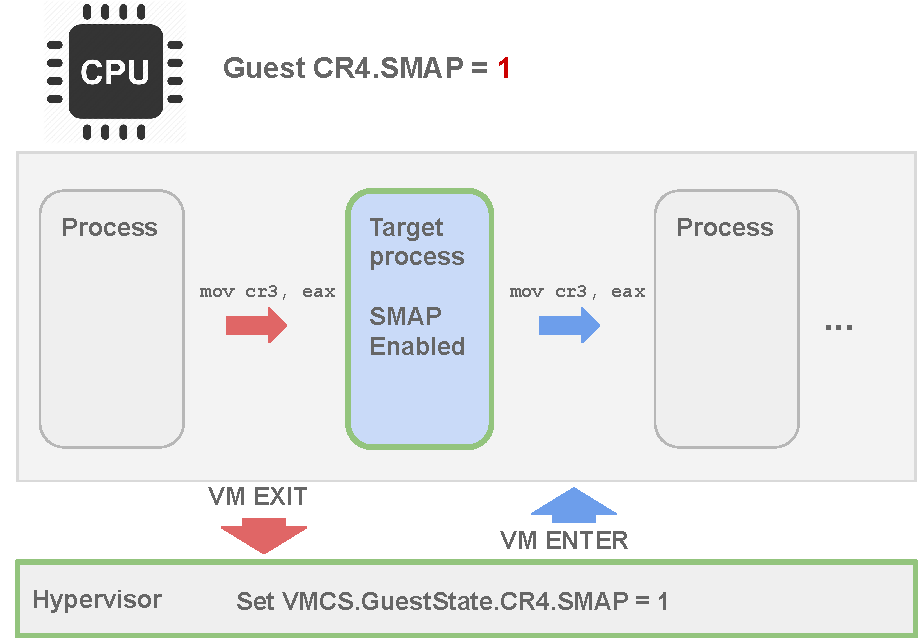
\includegraphics[width=0.40\textwidth]{figures/processmap3}
  \centering
  \caption{Operations on the CR3 register are the decisive characteristic of process context switching, which triggers VM exit by default. By setting the SMAP bit in the CR4 image of the VMCS.GuestArea, it updates the CPU CR4 when the hypervisor enters the virtual machine again. Therefore, it is possible to use the hypervisor to enable the SMAP feature when a specific process is running on the CPU.}
  \label{fig:processmap}
\end{figure}


By monitoring the process context switch event, namely, operations on the CR3 register, the hypervisor can temporarily enable/disable the SMAP feature to make it only active on a specific process. That is when this process is running on the CPU. As shown in~\autoref{fig:processmap}, \texttt{mov cr3, eax} triggers a VM Exit event, and the hypervisor receives it. If the new CR3 is one of the target processes, the hypervisor sets the CR4.SMAP in the Virtual Machine Control Structure (VMCS) of the guest virtual machine. It is the data structure that updates the real CPU registers when entering the virtual machine. Back to the guest, the SMAP is active while the process is running. When this process is switching out, the hypervisor again receives the event regarding CR3 operation. It then unset CR4.SMAP. Therefore, this particular process will have the illusion that SMAP is active continually while others feel the opposite.

The hypervisor inevitably brings performance overhead. However, it makes the mitigation more configurable. Due to the nature of local privilege escalation attacks, system processes already with high privilege are not likely threats. Hence no protection on them, which reduces the overall overhead.  Additionally, as previously mentioned, to prevent SMAP recurring caused dead loop, the feature isolation is also necessary. Therefore we consider the hypervisor framework as one contribution of this paper.
